
\subsubsection*{Geometry of Minkowski space}
Let $(\R^{1 + d}, \bfm)$ denote $(1 + d)$-dimensional Minkowski space with the usual metric, which in rectilinear coordinates $(t, x^1, \dots, x^d)$ takes the diagonal form 
	\[ 
		\bfm = - (\d t)^2 + (\d x^1)^2 + \dots + (\d x^d)^2. 
	\]
We will often write $t = x^0$ for the time coordinate and $x = (x^1, \dots, x^d)$ for the spatial coordinates. We reserve Greek indices, such as $\alpha, \beta, \gamma, \dots$ for space-time coordinates $(t, x^1, \dots, x^d)$, while Latin indices, such as $i, j, k, \ell,\dots$ will be reserved for spatial coordinates $(x^1, \dots, x^d)$. Another useful choice are the polar coordinates $(t, r, \Theta)$ where $r = |x|$ denotes the radius from the origin, and $\Theta := x/|x|$ denotes the radial projection onto the unit sphere $\SS^{d - 1}$. In these coordinates, the Minkowski metric takes the form 
	\[
		\bfm = - \d t^2 + \d r^2 + r^2 g_{\SS^{d - 1}}.
	\]
Denote $\partial_r = \tfrac{x^j}r \partial_j$ the radial vector field and $\nabla_{\SS^{d - 1}}$ for the gradient on the unit sphere $\SS^{d - 1}$. 

\subsubsection*{Geometry of the light cone}

We now introduce notation for the geometry of the light cone and subsets thereof. First and foremost, the forward light cone is defined by 
	\[
		C := \{ (t, x) \in [0, \infty) \times \R^d : r \leq t \}. 
	\]
When studying the light cone, it is convenient to work in null coordinates $(u, v, \Theta)$ defined by $u = t - r$ and $v = t + r$. In these coordinates, the Minkowski metric takes the form 
	\[
		\bfm = - \d u \d v + r^2 g_{\SS^{d -1}}.
	\]
The coordinate vector fields $L = \partial_t + \partial_r = 2 \partial_v$ and $\underline L = \partial_t - \partial_r = 2 \partial_u$ are referred to as null vector fields, as they are parallel to the forward and backwards light cones respectively. Observing that the forward light cone is foliated by surfaces
	\[
		\HH^d_{\rho} := \{ (t, x) \in [0, \infty) \times \R^d : t^2 + r^2 = \rho^2 \},
	\]
we introduce hyperbolic coordinates $(\rho, y, \Theta)$ where $\rho = \sqrt{t^2 - r^2}$ and $y = \tanh^{-1} (r/t)$. Each surface $\HH^d_\rho$ is isometric to the simply connected space of constant sectional curvature $-\tfrac{1}{\rho^2}$. In these coordinates the Minkowski metric takes the form 
	\begin{align*}
		\bfm 
			&= - \d \rho^2 + \rho^2  g_{\HH^d_\rho}\\
			&= - \d \rho^2 + \rho^2 (\d y^2 + \sinh^2 (y) g_{\SS^{d - 1}}).
	\end{align*}
We refer to the vector field $S = \rho \partial_\rho = x^\mu \partial_\mu$ as the scaling vector field, as it is generated from the scaling symmetry of the linear wave equation. 

	\begin{figure}[ht]
		\begin{center}
			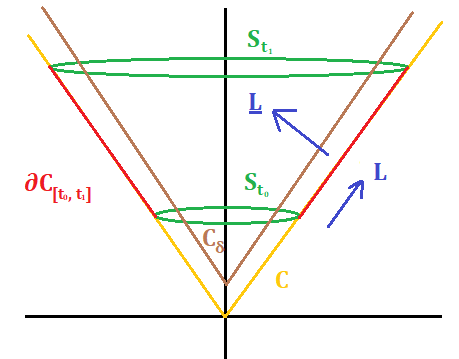
\includegraphics{graphics/cone}
			\caption{The geometry of the light cone. As a wise man once said, a picture is worth $\tfrac1\epsilon$-words for $\epsilon \ll 1$. }
		\end{center}	
	\end{figure}		

\subsubsection*{Subsets of $\R^d$ and $\R^{1 + d}$}
Define the restriction of the light cone to a time interval $I \subseteq [0, \infty)$ and a time slice $t \in [0, \infty)$ respectively by
	\begin{align*}
		C_I 
			&:= C \cap (I \times \R^d), \\
		S_{t}
			&:= C \cap (\{t\} \times \R^d).
	\end{align*}
The \emph{null boundary} $\partial C_I$ denotes the boundary of the time-slab $C_I$ modulo the top and bottom time-slices. Due to singularities on the null boundary, we will also consider the shifted light cone 
	\[ C^\delta := (\delta, 0) + C. \]
Accordingly, we have 
	\begin{align*}
		C^\delta_I
			&:= C_I \cap C^\delta, \\
		S^\delta_t
			&:= S_t \cap C^\delta.		
	\end{align*}	
We also define $B_r (x) \subseteq \R^d$ to be the ball of radius $r$ centered at $x$. 

